\newpage
\thispagestyle{empty}

\chapter{Results}

	\hspace{0.5cm} We've built an IoT-based automatic hand sanitizer dispenser with features including automatic refilling, hand sanitizer alerts, visitor counters and automatic dispensing.
	In the first step, we created a hand sanitizer dispenser with an    ultrasonic sensor that detects the user's hand. Sanitizer is dispensed as soon as hands are sensed. We created an alert system in which if anyone attempts to access the premises without sanitising their hands, a buzzer would beep continuously.Simultaneously, an alert SMS is sent to the registered mobile number. 
	After that, we built a bidirectional visitor counter to keep track of the number of persons entering and exiting the building, or in other words, the number of people present inside the building. We created an automated sanitizer refilling device at the end of the project. This feature automatically refills the sanitizer bottle when it reaches a certain level.
	
\newpage

	\begin{figure}[h]
		\centering
	\includegraphics[width=80mm,scale=1]{result1}
	\caption{Project Model}
	\label{Project Model}
	
\end{figure}

\vspace{1cm}
	\begin{figure}[h]
		\centering
	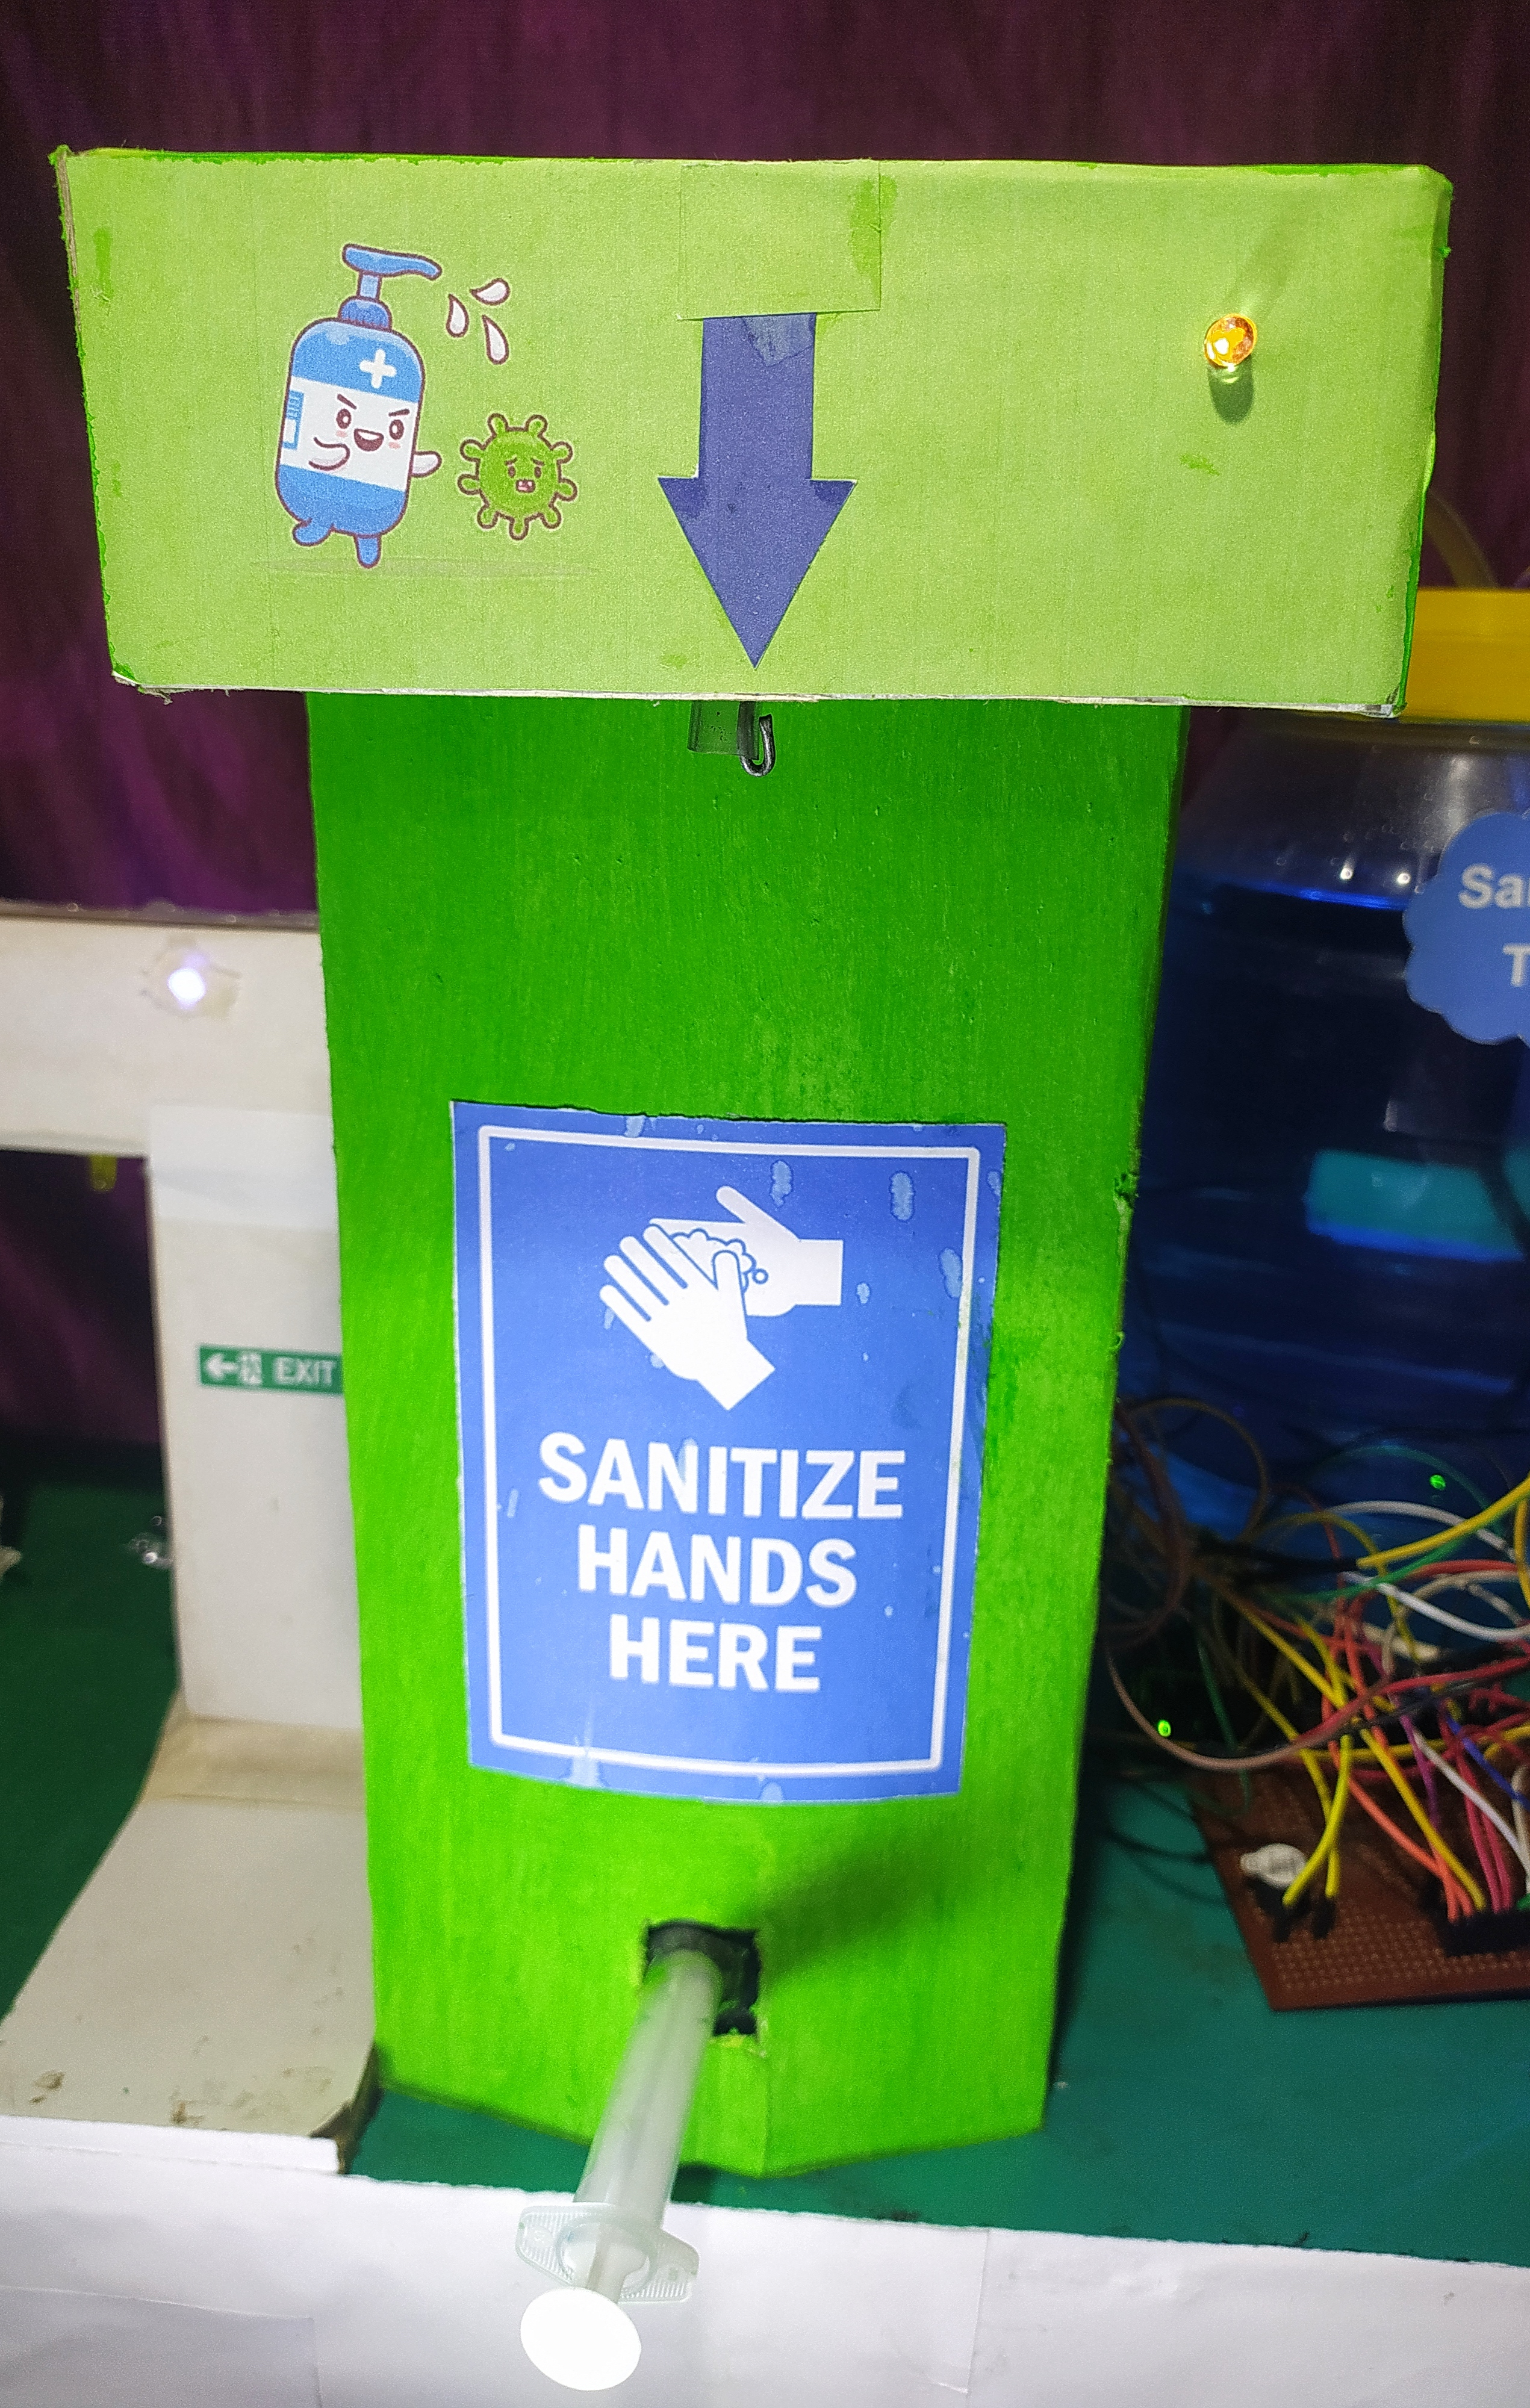
\includegraphics[width=45mm,scale=1]{result2}
	\caption{Sanitizer Dispenser}
	\label{Sanitizer Dispenser}
	
\end{figure}

\newpage

	\begin{figure}[h]
		\centering
	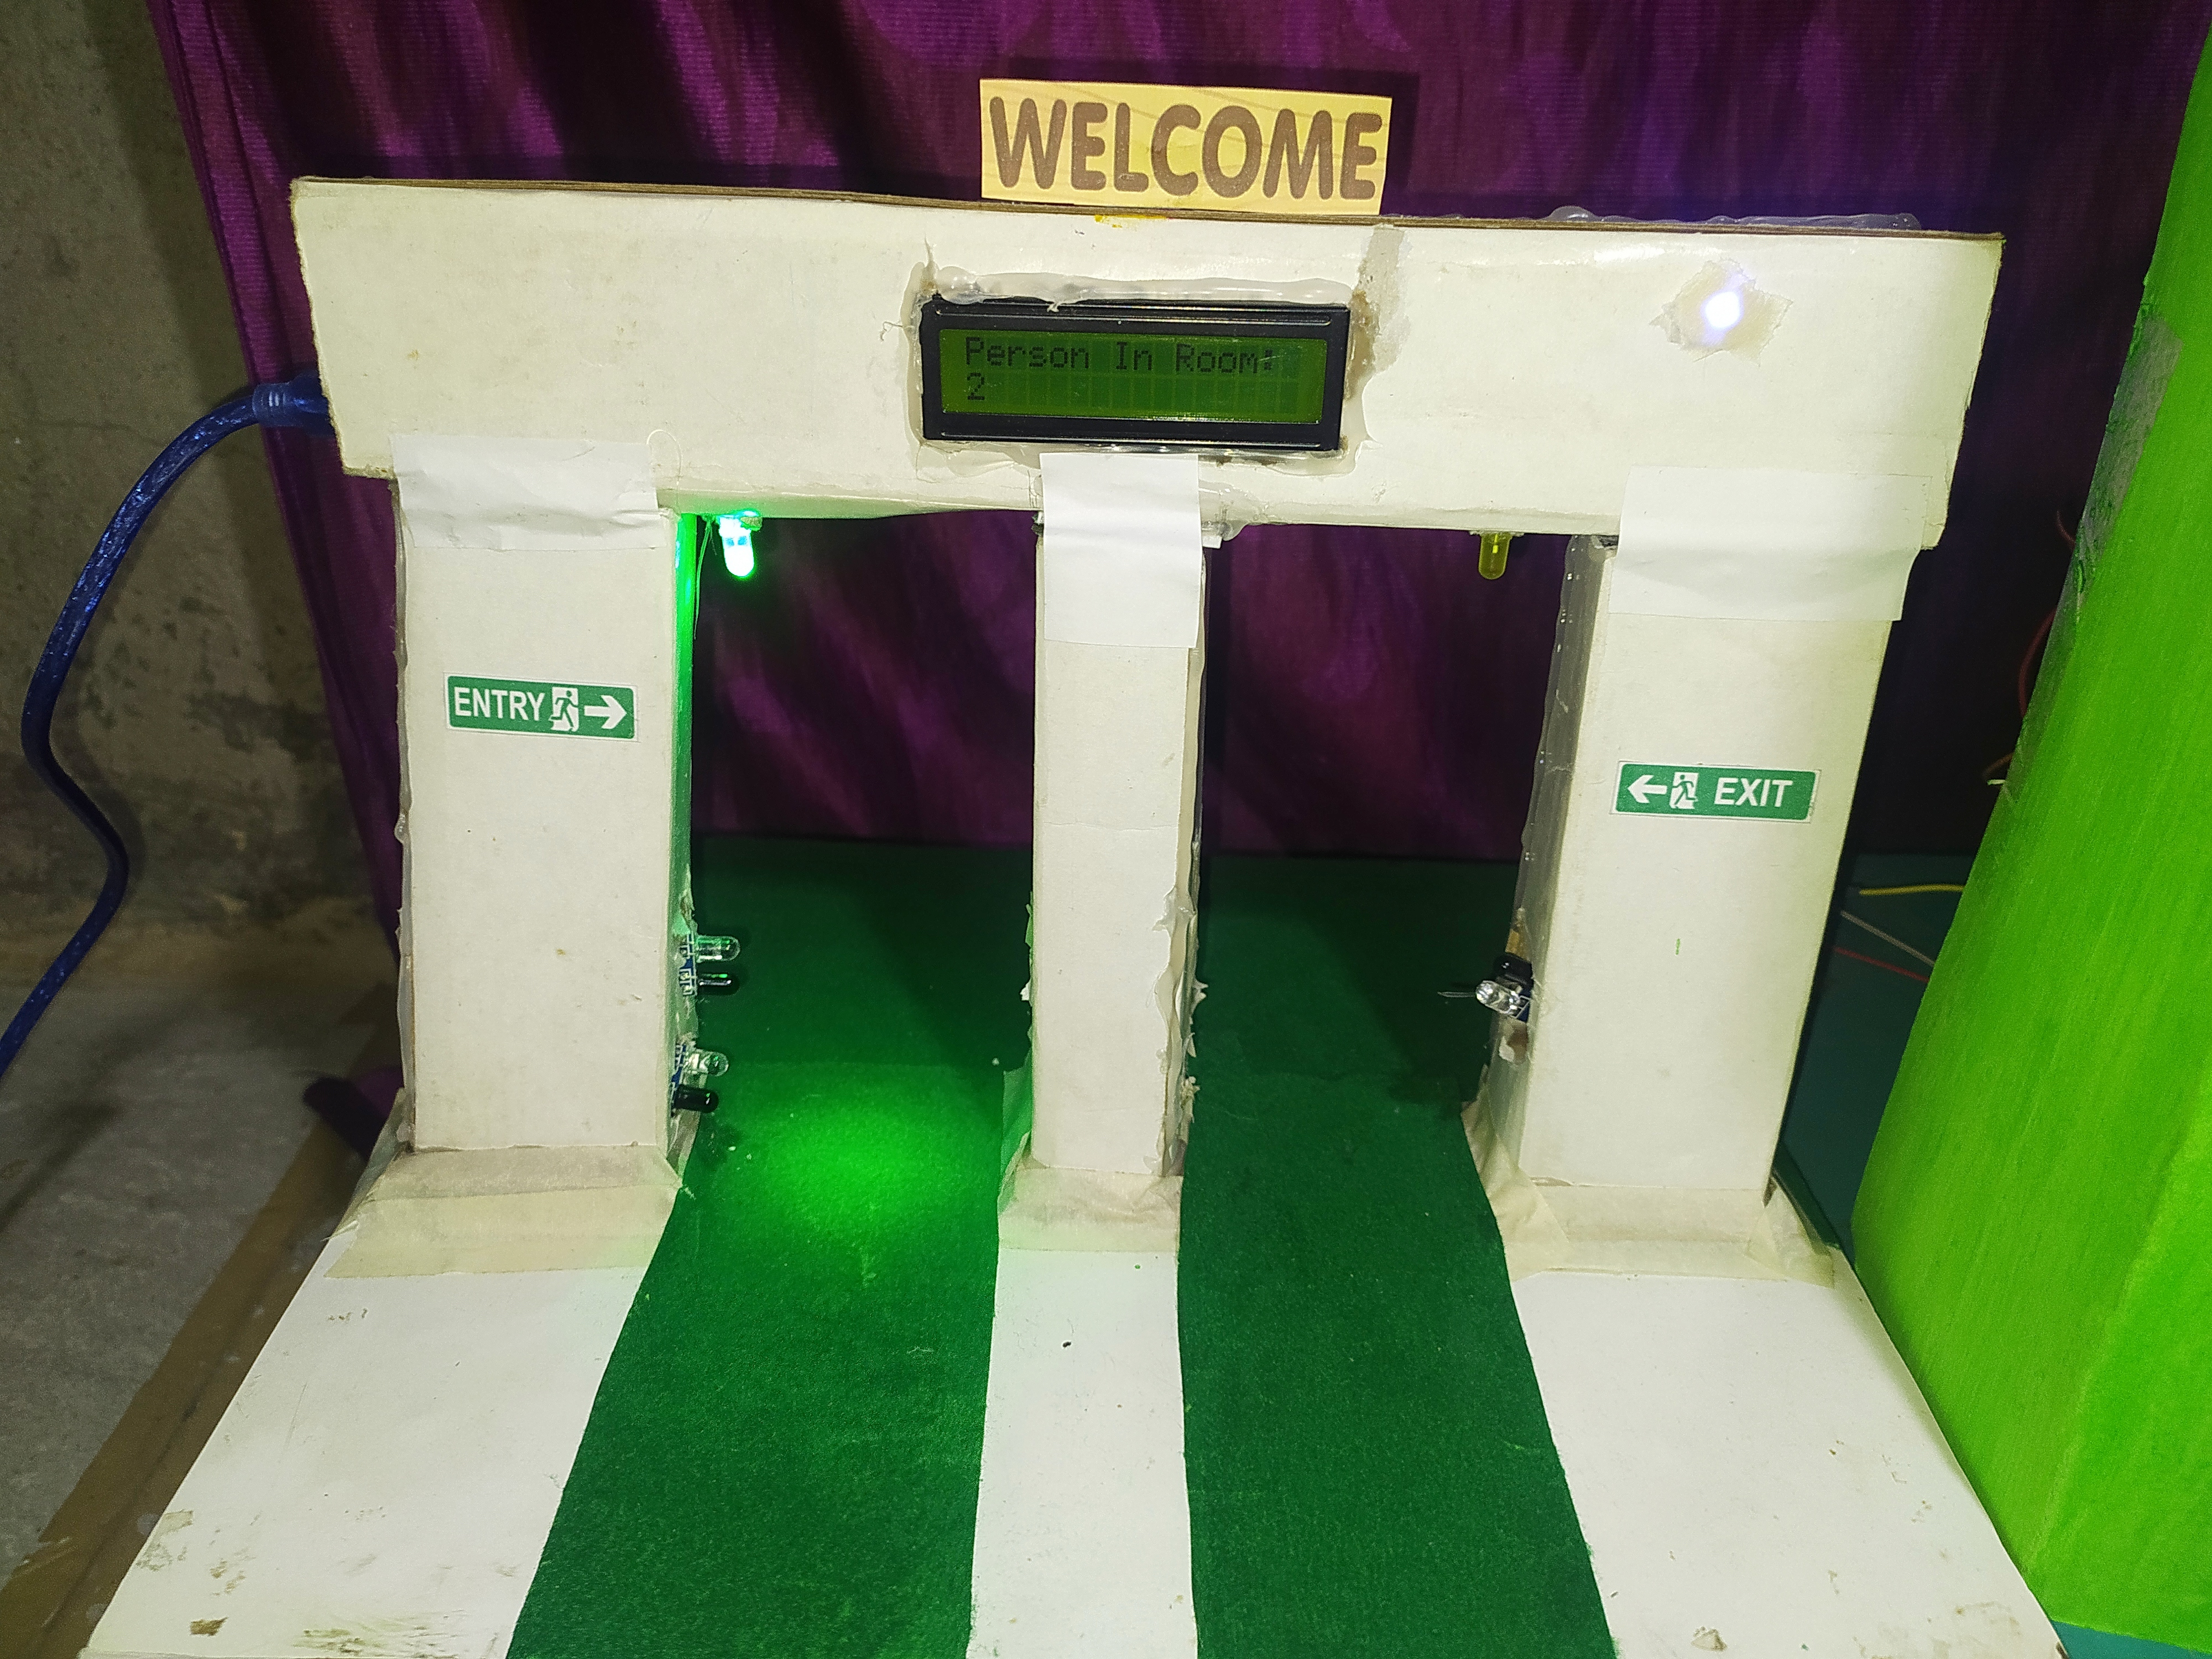
\includegraphics[width=75mm,scale=1]{result3}
	\caption{Bidirectional Visitor Counter}
	\label{Bidirectional Visitor Counter}
	
\end{figure}

\vspace{1cm}
	\begin{figure}[h]
		\centering
	\includegraphics[width=75mm,scale=1]{result4}
	\caption{Automatic tank filling system}
	\label{Automatic tank filling system}
	
\end{figure}

\newpage

	\begin{figure}[h]
		\centering
	\includegraphics[width=80mm,scale=1]{result5}
	\caption{Visitor Counter Display}
	\label{Visitor Counter Display}
	
\end{figure}

\vspace{1cm}
	\begin{figure}[h]
		\centering
	\includegraphics[width=41mm,scale=1]{result6}
	\caption{Alert SMS}
	\label{Alert SMS}
	
\end{figure}

